\chapter{Examples}
\label{c:examples}

An example of figures was shown in Fig.\ \ref{fig:dummy1}, and here are some
display style equations:

\begin{equation*}
	i \hbar \pdv[]{}{t} \Psi (x, t) = \left[ -\frac{\hbar^2}{2m} \pdv[2]{}{x}
	+ V(x, t) \right] \Psi (x, t)
\end{equation*}
\begin{equation*}
	H_{SO} = - \frac{\hbar}{4 m_0^2 c^2} \boldsymbol{\sigma} \cdot \boldsymbol{p}
	\times \grad V_0
\end{equation*}


and here's some inline math: $ e^{\pi i} + 1 = 0$.


\begin{figure}[bt]
	\centering
	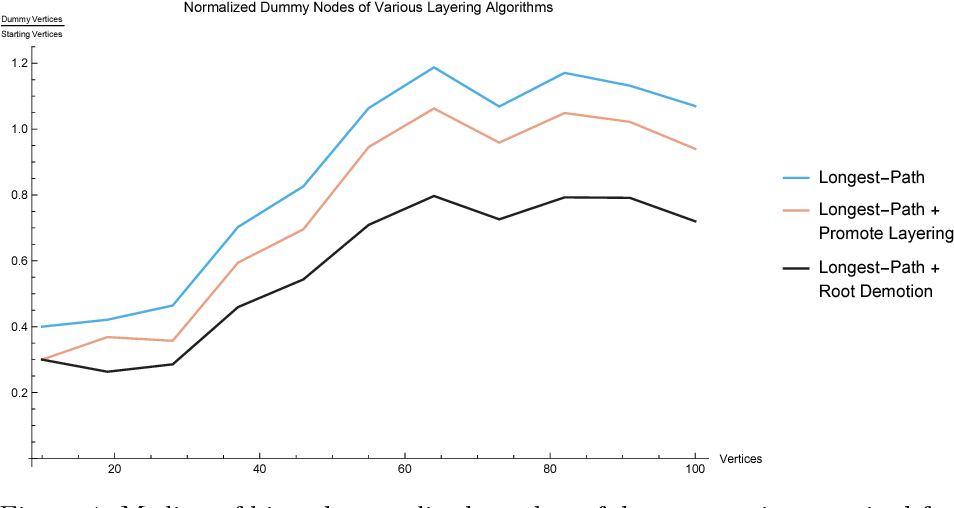
\includegraphics[width=0.6\linewidth]{./figures/dummy1.png}
	\caption{Dummy figure 1}%
	\label{fig:dummy1}
\end{figure}

\noindent Here are some citations \cite{einstein, latexcompanion}, and another 
example of display math \cite{knuthwebsite}:

\begin{table}[tb]
\centering
\caption{Dummy table}
\label{tab:dummy_tab}
\begin{tabular}{ |p{3cm}||p{3cm}|p{3cm}|p{3cm}|  }
 \hline
 \multicolumn{4}{|c|}{Country List} \\
 \hline
 Country Name     or Area Name& ISO ALPHA 2 Code &ISO ALPHA 3 Code&ISO numeric Code\\
 \hline
 Afghanistan   & AF    &AFG&   004\\
 Aland Islands&   AX  & ALA   &248\\
 Albania &AL & ALB&  008\\
 Algeria    &DZ & DZA&  012\\
 American Samoa&   AS  & ASM&016\\
 Andorra& AD  & AND   &020\\
 Angola& AO  & AGO&024\\
 \hline
\end{tabular} 
\end{table}

\begin{equation}
	\int_{-\infty}^\infty e^{-x^2} \dd x = \sqrt{\pi}
\end{equation}

Finally we have some code: \texttt{This is a demo of mono font}, and some
Sans Serif font: \textsf{Sans Serif}.

